%----------------------------------------------------------------------------
\chapter{\AudioBasics}
%----------------------------------------------------------------------------

\begin{comment} 
Annak érdekében, hogy a későbbi fejezetekben a hangtechnikai rendszerek működését és tervezését megérthessük,
először szükséges a hangtechnikai alapok ismerete. Ez a fejezet a későbbi fejezetekben használt alapfogalmakat definiálja röviden és tömören.

%----------------------------------------------------------------------------
\section{Mikrofon típusok}
%----------------------------------------------------------------------------

A mikrofon egy eszköz, amely az akusztikus energia hangterét elektromos energiává alakítja át.
Az eszköz érzékelheti a hangnyomást vagy a hangnyomás gradienst, amely arányos a hangsebességgel (mindkettő kombinációja a hangintenzitásnak).
Négy különböző átalakítótípus létezik, amelyeket reciprok transzducerekként használhatunk mikrofonokhoz:

% ----------------------------------------------------------------------------
\begin{itemize}
    \item Kapacitív transzducer
    \item Piezoelektromos transzducer
    \item Dinamikus transzducer
    \item Mágneses transzducer
\end{itemize}
% ----------------------------------------------------------------------------

Az említett összes transzducer lehetővé teszi a mechanikai rezgések elektromos rezgésekké történő átalakítását,
miközben különböző elveket követnek. Az első kettő esetében az elektromos mező változása
van használatban, míg az utolsó kettő esetében egy vezetőben keletkező áram indukciója a mágneses térben történő vezetékmozgás révén,
vagy a mágneses fluxus változása egy tekercsen. 
Elsősorban a négy említett transzducer közül kettőt a kapacitív és a dinamikus transzducert
használjuk gyakorlati jelentőséggel a rendezvénytechnikában.

% ----------------------------------------------------------------------------
\subsection{Dinamikus mikrofon}
% ----------------------------------------------------------------------------

A dinamikus mikrofonok a legelterjedtebb mikrofonok a hangtechnikában.
A hangnyomás mechanikai rezgéseit alakítják elektromos jelekké, elve, hogy egy membrán mely egy tekercsre van rögzítve, és ez mágneses mezőben mozog.
A membrán rezgése a tekercsben elektromos feszültséget indukál, amely a hangjelet reprezentálja.
Nagyon strapabíróak és megbízhatóak, széles körben használják őket élő hangosításban és stúdiótechnikában.
Hátránya a kisebb frekvenciaátvitel és a nagyobb torzítás.
Az egyik legismertebb dinamikus mikrofon a Shure SM57, amely egy nagyon népszerű mikrofon a hangtechnikában, és sokféle alkalmazásban használják.

% ----------------------------------------------------------------------------
\begin{figure}[H]
    \centering
    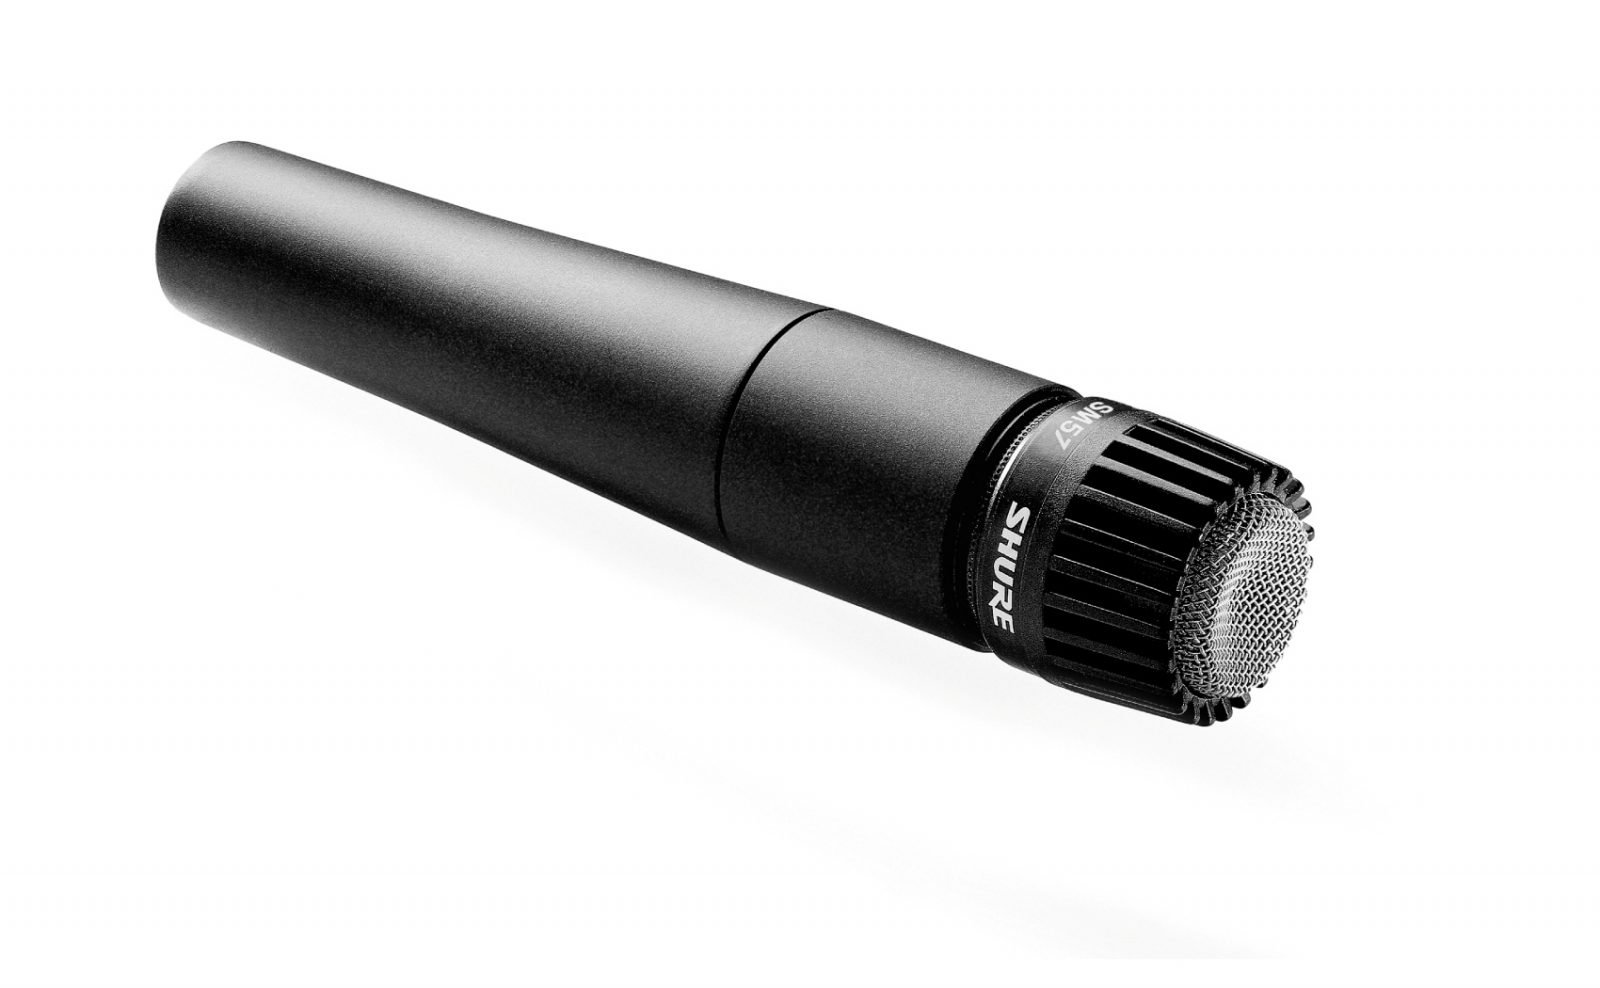
\includegraphics[width=0.3\textwidth]{figures/shure-sm57.jpg}
    \caption{Shure SM57 dinamikus mikrofon}
    \label{fig:shure_sm57}
\end{figure}
% ----------------------------------------------------------------------------

 
% ----------------------------------------------------------------------------
\subsection{Kondenzátor mikrofon}
% ----------------------------------------------------------------------------

A kondenzátor mikrofonok a nagyobb frekvenciaátvitellel rendelkező mikrofonok, és a nagyobb dinamikatartományt is képesek lefedni.
A hangnyomás a membrán rezgéseit egy kondenzátorban változó kapacitásként alakítja át, amelynek egyik eleme a membrán, a másik pedig egy fix elektromosan töltött lemez.
A membrán rezgései a kapacitás változását okozzák, amely a hangjelet reprezentálja.
A kondenzátor mikrofonok nagyon érzékenyek, és nagyon jó hangminőséget biztosítanak.
Azonban a kondenzátor mikrofonoknak van néhány hátránya is, például az áramellátás szükségessége, a magasabb ár és a nagyobb méretek.
Egy példa a kondenzátor mikrofonra a Shure SM137 kondenzátor mikrofon, amely egy elterjed mikrofon a hangtechnikában.

% ----------------------------------------------------------------------------
\begin{figure}[H]
    \centering
    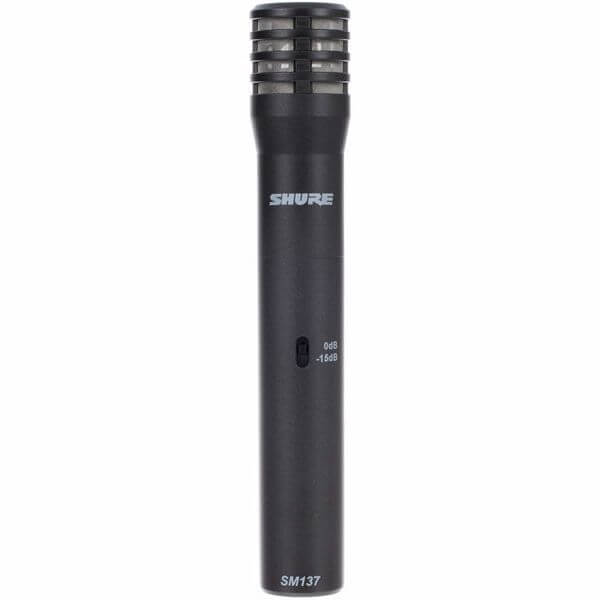
\includegraphics[width=0.3\textwidth]{figures/shure-sm137.jpg}
    \caption{Shure SM137 kondenzátor mikrofon}
    \label{fig:shure_sm137}
\end{figure}
% ----------------------------------------------------------------------------
\end{comment}

% ⛔📝 TODO: Merge text formatting and content integration check

%----------------------------------------------------------------------------
\section{Az analóg kezdetek} % Kezdeti analóg rendszerek, skálázhatósági hátrányok, analog rendszerek korlátai, működési alapelvek, technológiai háttér  
%----------------------------------------------------------------------------
Az analóg hangrendszerek története az audio technológia hajnalára nyúlik vissza. 
Az ilyen rendszerek alapját az elektromos analóg jelek képezik, amelyek az akusztikus hangot elektromos árammá alakítják,
a hangjelet közvetlenül, torzítás nélkül próbálják átadni az erősítőnek majd ezáltal hangszóróknak.
Az analóg rendszerek egyik legfontosabb alapelve az elektromos jelek folyamatos feldolgozása. 
A hangot analóg módon rögzítik, és az áramkörök szigorú tervezése biztosítja, hogy az eredeti akusztikus jel minél pontosabban tükröződjön az outputban.
A legnagyobb hátrány az analóg rendszerek skálázhatóságában rejlik. 
Ahogy a rendszer bonyolultsága nőtt, úgy a karbantartás és az állandó finomhangolás is egyre több problémát okozott. 
Az analóg technológiáknál a jel erősítése és kezelése gyakran jelentős torzulásokat és zajokat okozott, amelyeket nehéz volt kezelni.
A kábelezést tekintve sem volt egy leányálom az analóg rendszerek használata, mivel a nagyobb távolságokon a jel torzulása és a zajok könnyen bekerülhettek a rendszerbe.
Egy sokcsatornás produkciónál szép spagettiláncokat is eredményezett, még a legtapasztaltabb hangmérnökök számára is kihívást jelentett. 
Továbbá, a rendszer hibái nem mindig voltak könnyen diagnosztizálhatók, ami a szervizelési időket jelentősen megnövelte.
A hangrendszerek technológiai hátterét tekintve, az analóg rendszerekben a transzformátorok, kondenzátorok és ellenállások kulcsszerepet játszottak. 
Ezek az alkatrészek feleltek a jel szűréséért, erősítéséért és átalakításáért. 
Azonban ezek az elemek gyakran voltak érzékenyek a környezeti hatásokra, mint például a hőmérséklet-ingadozások és a páratartalom, 
amelyek további kihívások elé állították a hangmérnököket.
%----------------------------------------------------------------------------
\section{Digitális térhódítás} % Miért digitális irányba fejlesztünk és halad az ipar? Miért jobb mint az analog? 
%----------------------------------------------------------------------------
A digitális technológia térhódítása a professzionális audio rendszerekben jelentős paradigmaváltást hozott az audioiparban. 
Az utóbbi évtizedekben a digitális rendszerek folyamatosan felváltották az analóg megoldásokat, számos előnnyel rendelkezve, 
amelyek hozzájárultak a hangtechnikai rendszerek fejlődéséhez. 
Az egyik legfontosabb tényező, amely a digitális technológia előnyére szolgál, a jelminőség és a stabilitás drasztikus javulása. 
A digitális rendszerekben a hangjelek bitstream formájában kerülnek feldolgozásra, amely lehetővé teszi a zajok és torzítások minimalizálását,
a jelfeldolgozás során. 

A digitális rendszerek jelentős előnye, hogy magasabb jel-zaj viszonyt biztosítanak, amely fokozza a jel tisztaságát és mérsékli a zavaró hatásokat. 
Ezáltal a hangminőség jelentős javuláson megy keresztül, mivel a digitális feldolgozás során a hasznos jel és a 
háttérzaj közötti különbség egyértelműbbé válik.
Szélesebb dinamikatartományt nyújt, amely lehetővé teszi a nagyobb hangerő eltérések hatékony kezelését. 
A digitális rendszerek egyik további előnye, hogy a digitális adatok másolása során nem történik minőségromlás. 
A másolatok pontosan ugyanolyan minőséget képviselnek, mint az eredeti felvétel, így garantált a tökéletes reprodukálás.
Stabil működést biztosítanak változó hőmérsékleti és tápfeszültség-ingadozások mellett. 
Az analóg rendszerek által okozott torzulások elkerülhetőek, így nincs jelen jeltorzulás a digitális rendszerekben.
Képesek kezelni az együttfutás és hangmagasság-ingadozás problémáit, amelyeket az analóg rendszerek nehezebben tudnak kezelni.
A digitális rendszerek emellett képesek visszaállítani az egyenfeszültségű jelkomponenseket, és biztosítják 
a lineáris frekvenciamenetet, amely pontos hangátvitelt eredményez. 
%----------------------------------------------------------------------------
\subsection{PCM - Pulse Code Modulation}
%----------------------------------------------------------------------------
A hangfrekvenciás jelek digitális feldolgozása a PCM (Pulse Code Modulation, impulzuskód-moduláció) elvén alapul. 
Ennek során az analóg jelet diszkrét impulzusok sorozatára bontják, ahol az impulzusok 
amplitúdóértékei bináris kódokkal kifejezett információt hordoznak.

A PCM jel előállítása az A/D (analóg-digitális) átalakításon keresztül történik. 
Az analóg jelek időbeli és értékbeli folytonossága diszkrét minták sorozatává alakul, 
miközben az információtartalom megőrzi az eredeti jelhez hasonló értékét. 
Ezt a mintavételi tételt (C. E. Shannon) bizonyította, amely alapján az eredeti jel 
visszaállítható információveszteség nélkül, ha a mintavételi frekvencia legalább 
kétszerese az analóg jel legmagasabb frekvenciájának.

Az analóg jelben előforduló maximális frekvenciát Nyquist frekvenciának nevezik. 
Ennek megfelelően a mintavételi frekvencia határozza meg a digitális hangfeldolgozó rendszer sávszélességét. 
Figyelembe véve, hogy a hangfrekvenciás jel felső határa 20 kHz, a hifi hangminőség eléréséhez a 
mintavételi frekvencia minimálisan 40 kHz-nél nagyobb kell hogy legyen. A digitális hangfeldolgozás során jellemző mintavételi frekvenciák az alábbiak:
%----------------------------------------------------------------------------
\begin{itemize}
    \item CD minőség: 44.1 kHz
    \item DVD minőség: 48 kHz
    \item Studio minőség: 96 kHz
    \item Ultra minőség: 192 kHz
\end{itemize}
%----------------------------------------------------------------------------
A digitális hangfelvételek bitmélysége az analóg jelből származó egyes minták tárolásához 
felhasznált számjegyek számát jelöli. A CD hangformátum esetében a szabványos bitmélység 16 bit, 
míg a mintavételi frekvencia 44,1 kHz. Ez azt jelenti, hogy másodpercenként 44 100 hangmintát rögzítenek, 
és minden egyes minta 16 bitnyi információt tartalmaz. 
Bár a nagyobb bitmélység általában jobb hangminőséget biztosít, ez egyúttal nagyobb fájlmérettel is jár.
A digitális hangfeldolgozás során jellemző bitmélységek az alábbiak:
%----------------------------------------------------------------------------
\begin{itemize}
    \item CD minőség: 16 bit
    \item Studio/live minőség: 24 bit
    \item Ultra minőség: 32 bit
\end{itemize}
%----------------------------------------------------------------------------
\begin{figure}[H]
	\centering
	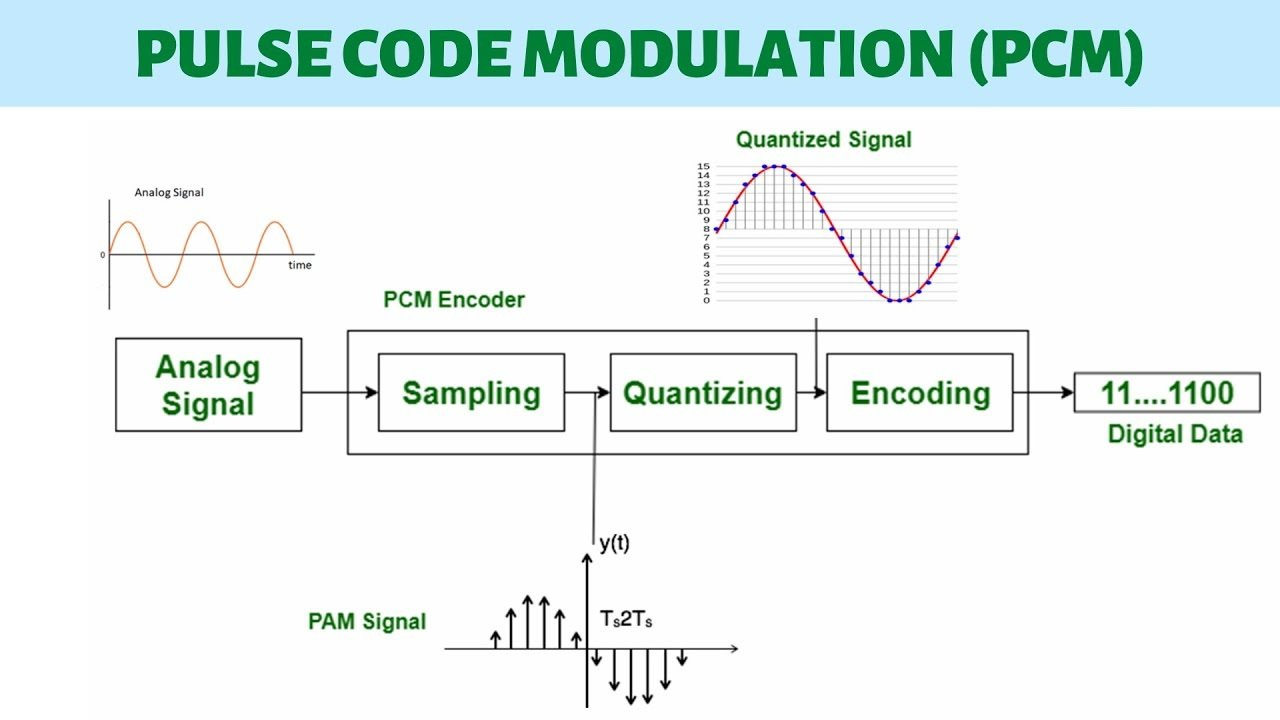
\includegraphics[width=\linewidth, keepaspectratio]{figures/pulse _code_modulation.jpg}
	\caption{Pulse Code Modulation (PCM) folyamat~\cite{PULSECODEMODULATION}}\label{fig:pcm}
\end{figure}
%----------------------------------------------------------------------------
A digitális hangfeldolgozás területén fontos szerepet játszik az A/D átalakítók kialakítása, 
a kódolás folyamata, a D/A (digitális-analóg) átalakítás, valamint a hibafelismerés és hibajavítás.
%----------------------------------------------------------------------------
\subsection{ADC és DAC konverterek - mintavételezés}
%----------------------------------------------------------------------------
A mintavételezés olyan folyamat, amely során egy analóg hangjeleket digitális formába alakítanak át, azaz mintákat vesznek az időben folytonos hanghullámokból. 
Ez az alapja annak, hogy a hangot számítógépes rendszerekben kezelni lehessen. A hangminták gyakorisága meghatározza a mintavételi frekvenciát, 
ami meghatározza a digitális hangminőséget és a frekvencia tartományt. Általában minél magasabb a mintavételi frekvencia, annál jobb a hangminőség, 
de nagyobb sávszélességet is eredményez.

A digitalizálási folyamat során az időbeli mintavételezés történik. 
Folyamatos mintavételezéskor a hang intenzitásával arányos diszkrét értékek, azaz feszültségimpulzusok jönnek létre. 
A mintavétel során az impulzusok a beérkező amplitúdó értékek alapján végtelen számú értéket vehetnek fel, 
ám a rendelkezésre álló bináris adatszók száma véges. Ezt a jelenséget kvantálásnak vagy tartományokba 
való felosztásnak nevezzük.

A kvantálás során a hangtartomány véges számú lépcsőre oszlik. 
A kvantálás finomsága, amely a mintavételi frekvenciával együtt a digitális jelfeldolgozás 
egyik legfontosabb paramétere, meghatározza a hang digitalizálásának részletességét. Gyakorlatilag a 
hangfrekvenciás jelek digitalizálásánál általában 14 vagy 16 bites kvantálást alkalmaznak. 
A kvantálásnál figyelembe kell venni a kvantálási zajt is, amely a tartományok növelésével csökkenthető.
A kvantálási zaj olyan zavaró tényező, amely a digitális hangrögzítés vagy -lejátszás során jelentkezik, 
és a kerekítési hibák következményeként alakul ki. Ez a zaj a különbség az eredeti analóg jel és a 
digitális formában ábrázolt jel értékei között, amit a digitális eszközök kvantálási folyamatában jelentkező pontatlanságok okoznak.
A kvantálási zaj keletkezése a digitális jel analóg formából történő diszkrét értékekre (kvantumokra) 
történő átalakítása során jelentkező kerekítési hibákra vezethető vissza. 
E hibák következtében a kvantálási zaj nemlineáris, hanem zavaró zajként észlelhető, 
amely nem harmonikus torzítás formájában jelenik meg, hanem inkább a hangminőség romlásához vezető zavaró tényezőként.

A kvantálási zaj csökkentésére több módszer létezik. Az egyik lehetséges megoldás a 
digitális jel dinamikatartományának növelése. Amennyiben a kvantálási pontosságot 
egy bittel növeljük, a jel-zaj viszony javulhat, és ezzel együtt a dinamika is +6 dB-el növekedhet. 
Továbbá, a zajcsökkentő algoritmusok alkalmazása és a magas felbontású digitális konverterek használata szintén hozzájárulhat a kvantálási zaj mérsékléséhez.
A kódolás során a hangszintek szerint kvantált pontok kódkombinációk sorozataként, digitális jelekként jelennek meg.

Az ADC (Analog-to-Digital Converter) konverter az analóg hangjeleket digitális jelekké alakítja át, míg a DAC (Digital-to-Analog Converter) 
konverter a digitális jeleket visszaalakítja analóg hangjelekké. 
A professzionális ADC és DAC konverterek nagymértékben befolyásolják a hangminőséget.
%----------------------------------------------------------------------------
\section{Hangerősség és hangnyomásszint} % Mi a hangerősség és a hangnyomásszint? Hogyan mérjük őket? Mi a különbség közöttük?
%----------------------------------------------------------------------------
Hangerőség (Intenzitás):
A hangerőség az a szubjektív hangosságérzet, amely a fizikai hangnyomás szintjétől függ. 
Ennek mértéke phonban van kifejezve, ahol a hangerőség értéke annyi phon, ahány dB-t mérünk 
egy 1 kHz-es szinuszhang hangnyomásszintjén, amely azonos hangosságérzetet kelt.

Hangosság (Hangnyomásszint):
A hangosság az egyidejűleg megszólaló hangok összefoglaló mértékét jelöli, amelyet a sone egységében mérünk. 
A kiszámítása során, ha a hangerőség meghaladja a 40 phon értéket, a hangosságot sone-ban adják meg.

A dB-skála a hangnyomásszint logaritmikus kifejezésére szolgál. Az emberi hallás érzékenysége különböző 
frekvenciákon eltérő, és a decibelskála lehetővé teszi, hogy az emberi hallás által 
érzékelhető hangnyomás tartományát pontosan ábrázoljuk.
A hangosság és a hangerőség közötti eltérés abban rejlik, hogy míg a hangosság az emberi érzékelésre, 
vagyis az érzékelhető hangnyomásra vonatkozik, addig a hangerőség a hanghullámok 
fizikai tulajdonságait, vagyis a hullámokban terjedő energiát méri.
%----------------------------------------------------------------------------
\begin{figure}[H]
	\centering
	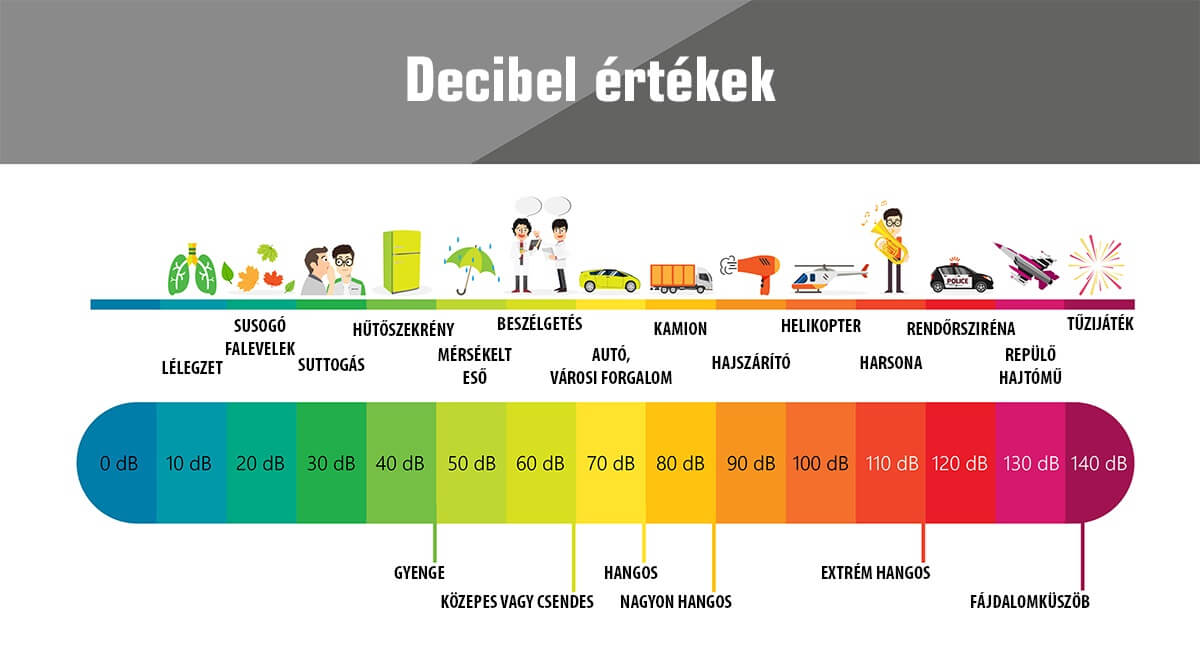
\includegraphics[width=\linewidth, keepaspectratio]{figures/db_scale.jpg}
    \caption{Decibel skála~\cite{DECIBELSCALE}}\label{fig:db_scale}
\end{figure}
%----------------------------------------------------------------------------
Az emberi fül által észlelt legkisebb hangerősség 0 dB, amely alig érzékelhető. 
A 50 dB körüli hangerőt kellemesnek találjuk, míg a 100 dB-es szint már kellemetlenséget 
okozhat. A fájdalomküszöb nagyjából 120 dB-nél helyezkedik el. Érdemes megjegyezni, hogy 
a 100 dB nem kétszerese az 50 dB-nek hangerősség szempontjából. A hangerő érzékelése 
szubjektív, és az egyéni hallási képességek határozzák meg. Általában egy 10 dB-es 
növekedést körülbelül kétszer olyan hangosnak érzékelünk, tehát egy 60 dB-es hangerőt 
körülbelül kétszer hangosabbnak érzünk, mint az 50 dB-eset. Mivel a decibelskála logaritmikus 
alapú, a dB-ben megadott értékek nem lineárisan arányosak. Például a 120 dB nem kétszerese 
a 60 dB-nek, hanem a hangnyomása hozzávetőlegesen ezerszer nagyobb. A hangnyomás mérésére 
különböző súlyozási görbéket alkalmazhatunk, például A, C és Z súlyozást. Mit is jelentenek 
ezek? Ha egy hang az összes frekvenciatartományban egyenlő hangnyomással rendelkezik, azt a 
Z-súlyozási görbe segítségével ábrázolhatjuk. Az emberi fül által észlelt hangokat az 
A-súlyozási görbe írja le, amely pontosan tükrözi az emberi hallás frekvenciatartományát, mivel 
az emberi hallás nem érzékel minden frekvenciát egyformán. A C-súlyozás a hangélményt 
reprezentálja, amikor a hangerő növekedésével az alacsonyabb frekvenciák iránti érzékenység is 
fokozódik. Az A- és C-súlyozás tehát a leginkább megfelelő az emberi hallás valósághű 
frekvenciaválaszának modellezésére.
%----------------------------------------------------------------------------
\begin{figure}[H]
	\centering
	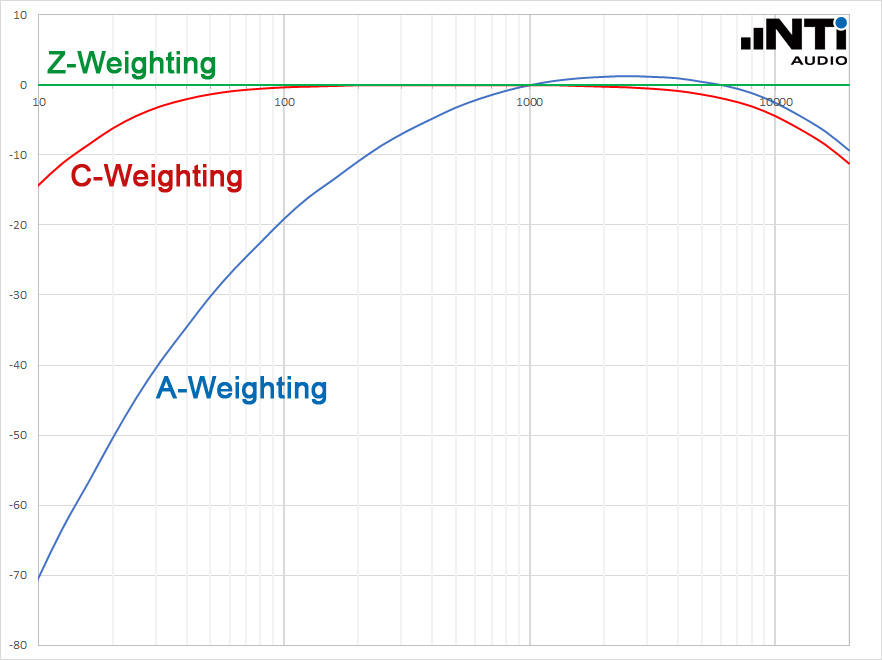
\includegraphics[width=\linewidth, keepaspectratio]{figures/db_weights.jpg}
    \caption{A-, C- és Z-súlyozás~\cite{DBWEIGHTS}}\label{fig:db_weights}
\end{figure}
%----------------------------------------------------------------------------
\newpage
\section{Pontsugárzó és LineArray hangforrások} % Mi a különbség a pontsugárzó és LineArray hangforrások között? Milyen alkalmazási területeken használjuk őket?
%----------------------------------------------------------------------------
Hangládák kiválasztásakor a legelterjedtebb formátumok a pontsugárzó és a Line Array rendszerek.
Ez a két típusú hangforrás eltérő működési elvekkel rendelkezik, 
amelyek befolyásolják megfelelő alkalmazási területeiket és a hangzás minőségét.
A pontsugárzó hangszórók, jellemzően kisebb eseményeken, 
otthoni környezetben és egyes konferenciákon találhatók meg. Ezek a hangszórók egyetlen 
dobozból állnak, amelyben minden szükséges komponens elhelyezésre került a hang előállításához. 
A pontsugárzók a hangot minden irányba terjesztik, olyan módon, mintha a hang egyetlen pontból áramlana ki. 
Könnyen telepíthetők és jól alkalmazhatók kisebb rendezvényekhez. Különböző méretűek 
lehetnek, a kis asztali hangszóróktól kezdve a nagyobb DJ-rendszerekig.
%----------------------------------------------------------------------------
\begin{figure}[H]
	\begin{minipage}{0.5\textwidth}
		\centering
		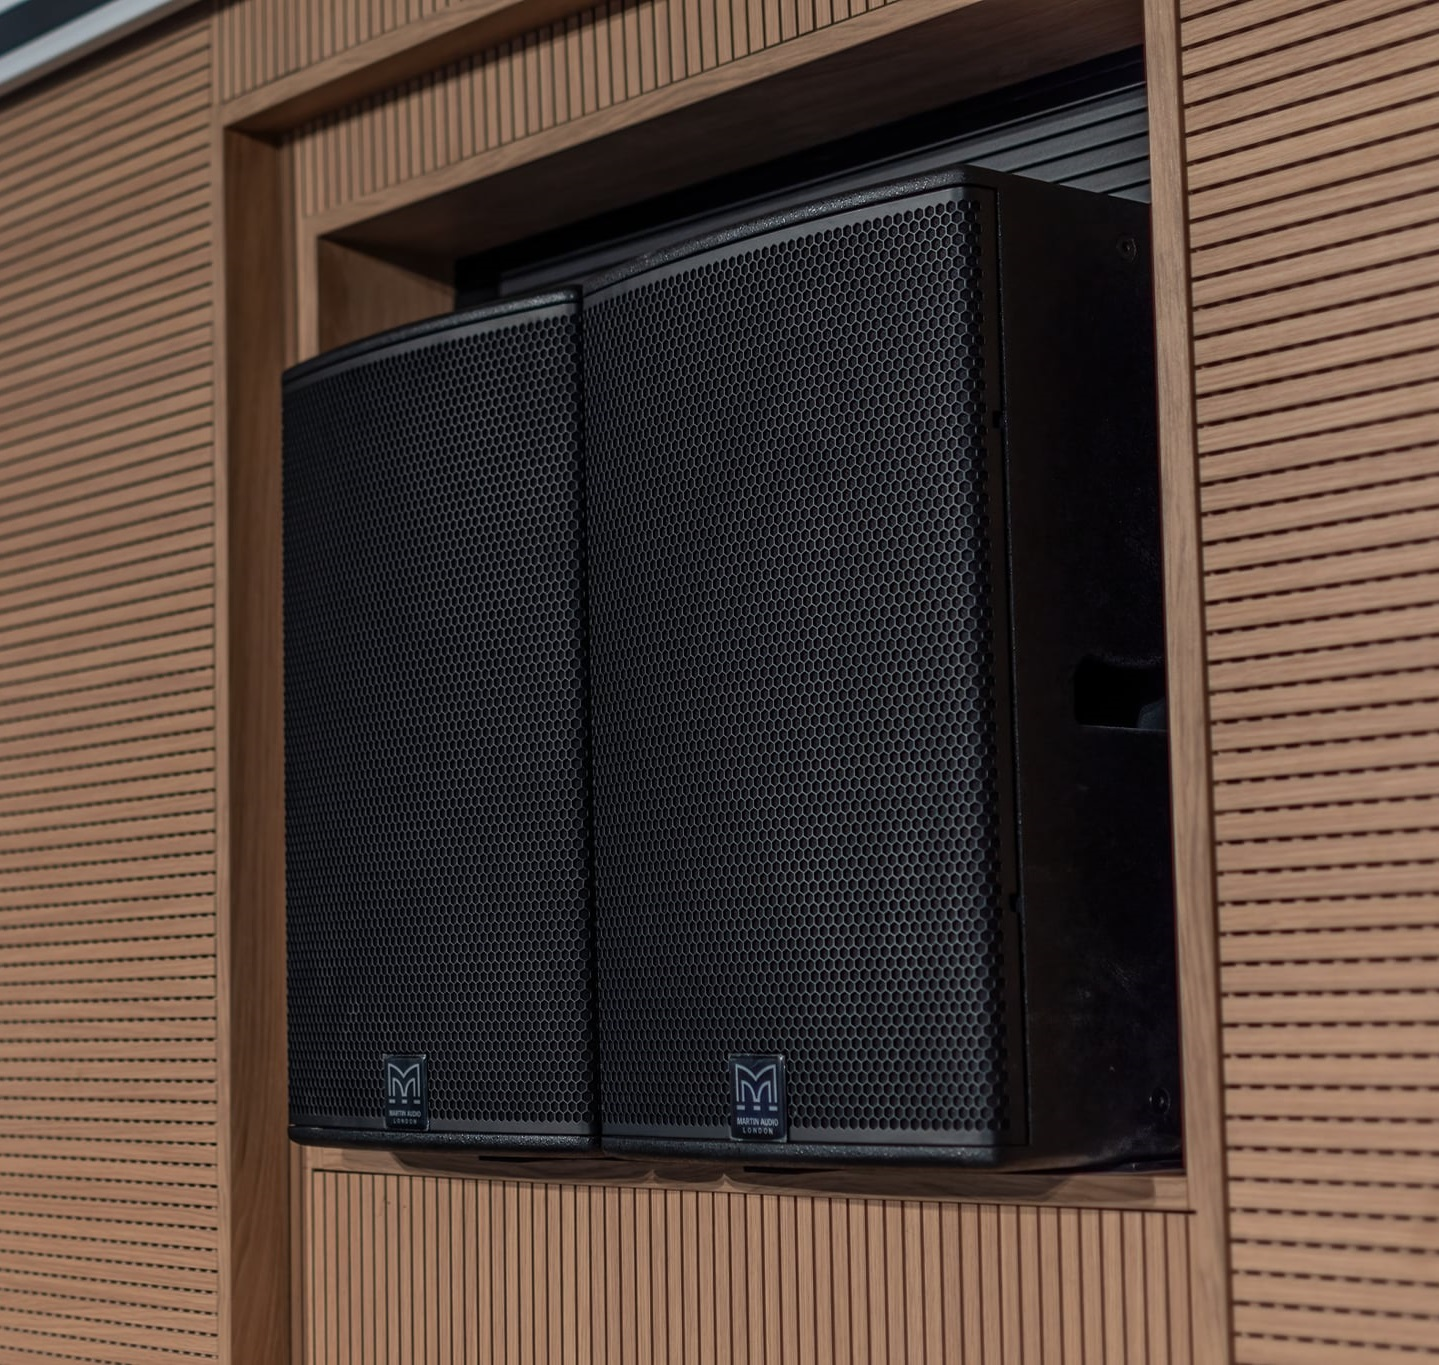
\includegraphics[width=200px, keepaspectratio]{figures/point_source.jpg}
        \caption{Pontsugárzó rendszer}
        \label{fig:point_source}
	\end{minipage}%
	\begin{minipage}{0.5\textwidth}
		\centering
		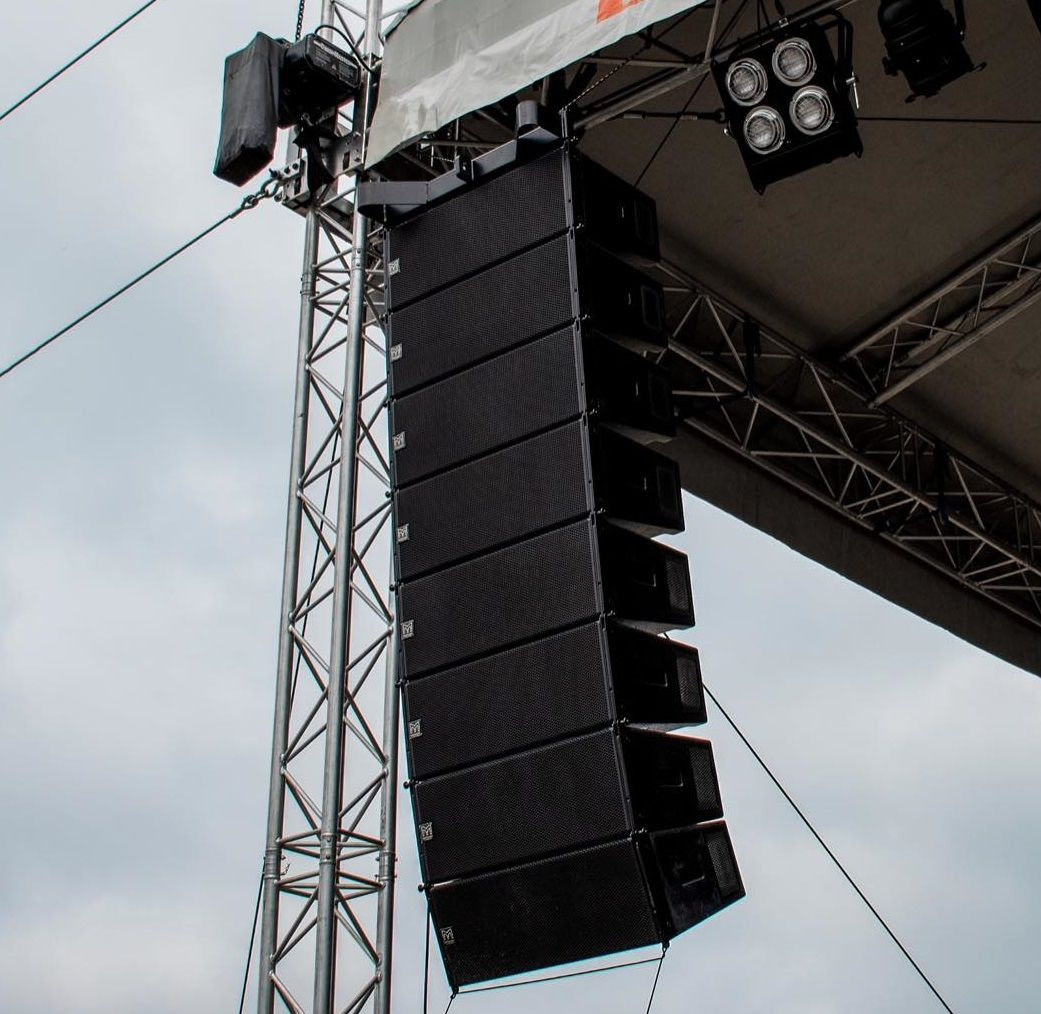
\includegraphics[width=200px, keepaspectratio]{figures/line_array.jpg}
		\caption{Line Array rendszer}
        \label{fig:line_array}
	\end{minipage}
\end{figure}
%----------------------------------------------------------------------------
A Line Array rendszerek ezzel szemben több dobozból állnak, amelyek egymáshoz képest függőlegesen vannak elrendezve.
Minden doboz több kisebb hangszórót tartalmaz. Amikor ezek a dobozok sorba vannak állítva, 
együtt működnek egy hatékony és kontrollált hangzás előállításában, amely sokkal könnyebben irányítható. 
A Line Array rendszerek ideálisak nagyobb eseményekhez vagy szabadtéri koncertekhez, mivel képesek 
nagyobb területet lefedni. Az ilyen rendszerek vezérlése lehetővé 
teszi olyan okos megoldások alkalmazását is, mint például a 'kizárási zónák' létrehozása, vagy a 
hang egy adott területre való fókuszálása a helyszínen.
Összefoglalva, a pontsugárzó és a Line Array hangszórók közötti alapvető különbség a hangterjesztés módjában rejlik. 
Míg a pontsugárzó hangszórók a hangot minden irányba szórják, addig a Line Array hangszórók a hangot meghatározott területekre irányítják. 
A pontsugárzók inkább kisebb rendezvényekhez ajánlottak, míg a Line Array rendszerek nagyobb helyszínekhez vagy szabadtéri eseményekhez ideálisak.
%----------------------------------------------------------------------------
\subsection{LineArray DSP-vezérelt irányítás~\cite{AHNERT2023}}
%----------------------------------------------------------------------------
A hangosító rendszerek tervezésének fő célja, hogy a közönség számára kiváló minőségű hangzást biztosítson. 
A kiváló hangzás alatt egyenletes hangerejű, homogén frekvenciaválaszú, alacsony torzítással rendelkező és mindenhol jól érthető hangot értünk. 
E célok elérése érdekében a modern lesugárzó rendszerek elektronikus úton állítható irányokkal rendelkeznek. 
Ehhez egyedi digitális jelkezelést (DSP) és egyedi erősítést alkalmaznak minden egyes meghajtóhoz.
%----------------------------------------------------------------------------
\begin{figure}[H]
    \centering
    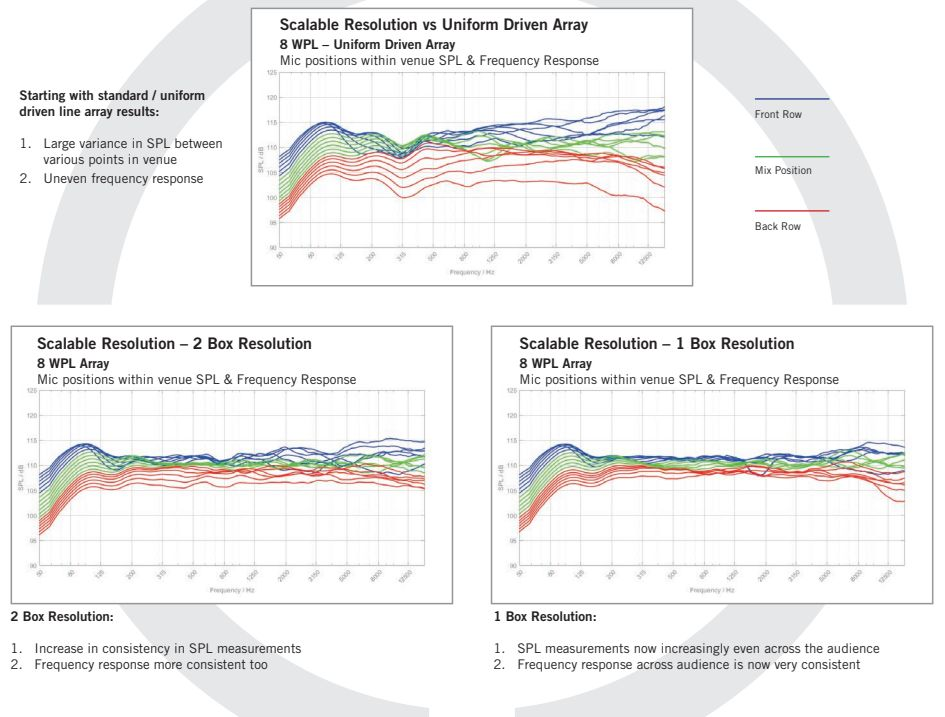
\includegraphics[width=\linewidth, keepaspectratio]{figures/dsp_arrays.jpg}
    \caption{DSP-vezérelt Line Array~\cite{AHNERT2023}}
    \label{fig:dsp_arrays}
\end{figure}
%----------------------------------------------------------------------------
A DSP-vezérelt line array hangszórók találmánya az 1990-es évekre nyúlik vissza, és azóta folyamatosan fejlődött.
Ma már számos gyártó kínál különböző méretű és felbontású DSP-vezérelt irányítható rendszereket, 
amelyek igyekeznek minden hangosítási igényt kielégíti. 
Különösen akusztikailag nehéz helyszíneken, ahol sok a reflektáló felület és nagy a visszhang effektus. 
Itt az ilyen vezérléssel rendelkező rendszerek teljesítménye egyértelműen felülmúlja a hagyományosak eredményeit. 
A DSP programozása speciális szoftvert igényel, amelyet a gyártó biztosít, és lehetővé tesz különböző szűrő paraméterek optimalizálását a kívánt irányítottság eléréséhez. 
Általában a cél egy keresztmetszeti tervként van meghatározva, és a line array rendszer irányítása ennek a célzott terület egyenletes lefedésére irányul.
A rendszerek tervezése számítógépes eszközöket igényel, amelyek lehetővé teszik a hangszórók viselkedésének részletes szimulációját, például hogyan reagál a térben egy bizonyos rendszer.